\documentclass[a4paper,11pt]{article}
\usepackage[utf8]{inputenc}
\usepackage[T1]{fontenc}
\usepackage[italian,english]{babel}
\usepackage{graphicx}
\usepackage[hidelinks]{hyperref}
\usepackage{geometry}
\usepackage{float}

\geometry{margin=2.5cm}

\title{Data Warehouse Report}
\author{Pierpaolo Spadafora - 263722}
\date{\today}

\begin{document}

\maketitle

\section{Introduction}

I chose the \textbf{Online Sales Dataset}\footnote{\url{https://www.kaggle.com/datasets/yusufdelikkaya/online-sales-dataset}} which is a sample e-commerce database on Kaggle.
To support richer analytics the data warehouse includes economic indicators such as \textit{Gross Domestic Product} (GDP) \footnote{\url{https://data.worldbank.org/indicator/NY.GDP.MKTP.KD}} and \textit{GDP per capita}\footnote{\url{https://data.worldbank.org/indicator/NY.GDP.PCAP.CD}} provided from the World Bank.\\
The aim is to provide multidimensional analytical perspectives relating sales performance to geographical context and economic trends, at a good level of quality, consistency and detail.

\section{Dataset Analysis and Preparation}
\subsection{Primary Dataset Overview}
The Online Sales Dataset consists of \textbf{49,782 records} across \textbf{17 columns}, covering the period from \textit{January 2020} to \textit{September 2025}. Key attributes include:
\begin{itemize}
    \item \textbf{Transaction details}: \texttt{InvoiceNo}, \texttt{InvoiceDate}, \texttt{CustomerID}, \texttt{Discount},
    \item \textbf{Product information}: \texttt{StockCode}, \texttt{Description}, \texttt{Category}, \texttt{UnitPrice}, \texttt{Quantity},
    \item \textbf{Geographic and operational data}: \texttt{Country}, \texttt{SalesChannel}, \texttt{ShipmentProvider}, \texttt{OrderPriority}, \texttt{ReturnStatus}
    \item \textbf{Financial and logistical metadata}: \texttt{ShippingCost}, \texttt{PaymentMethod}, \texttt{WarehouseLocation}
\end{itemize}

\subsection{Economic Indicators Integration}

The World Bank economic datasets contains GDP and GDP per capita indicators in current US dollars for 266 countries from 1960 to 2024. 
The original dataset is structured as:\\
\texttt{"Country Name","Country Code","Indicator Name","Indicator Code","1960","1961",...,"2024"}

\subsection{Data Quality Assessment}
\begin{figure}[H]
    \centering
    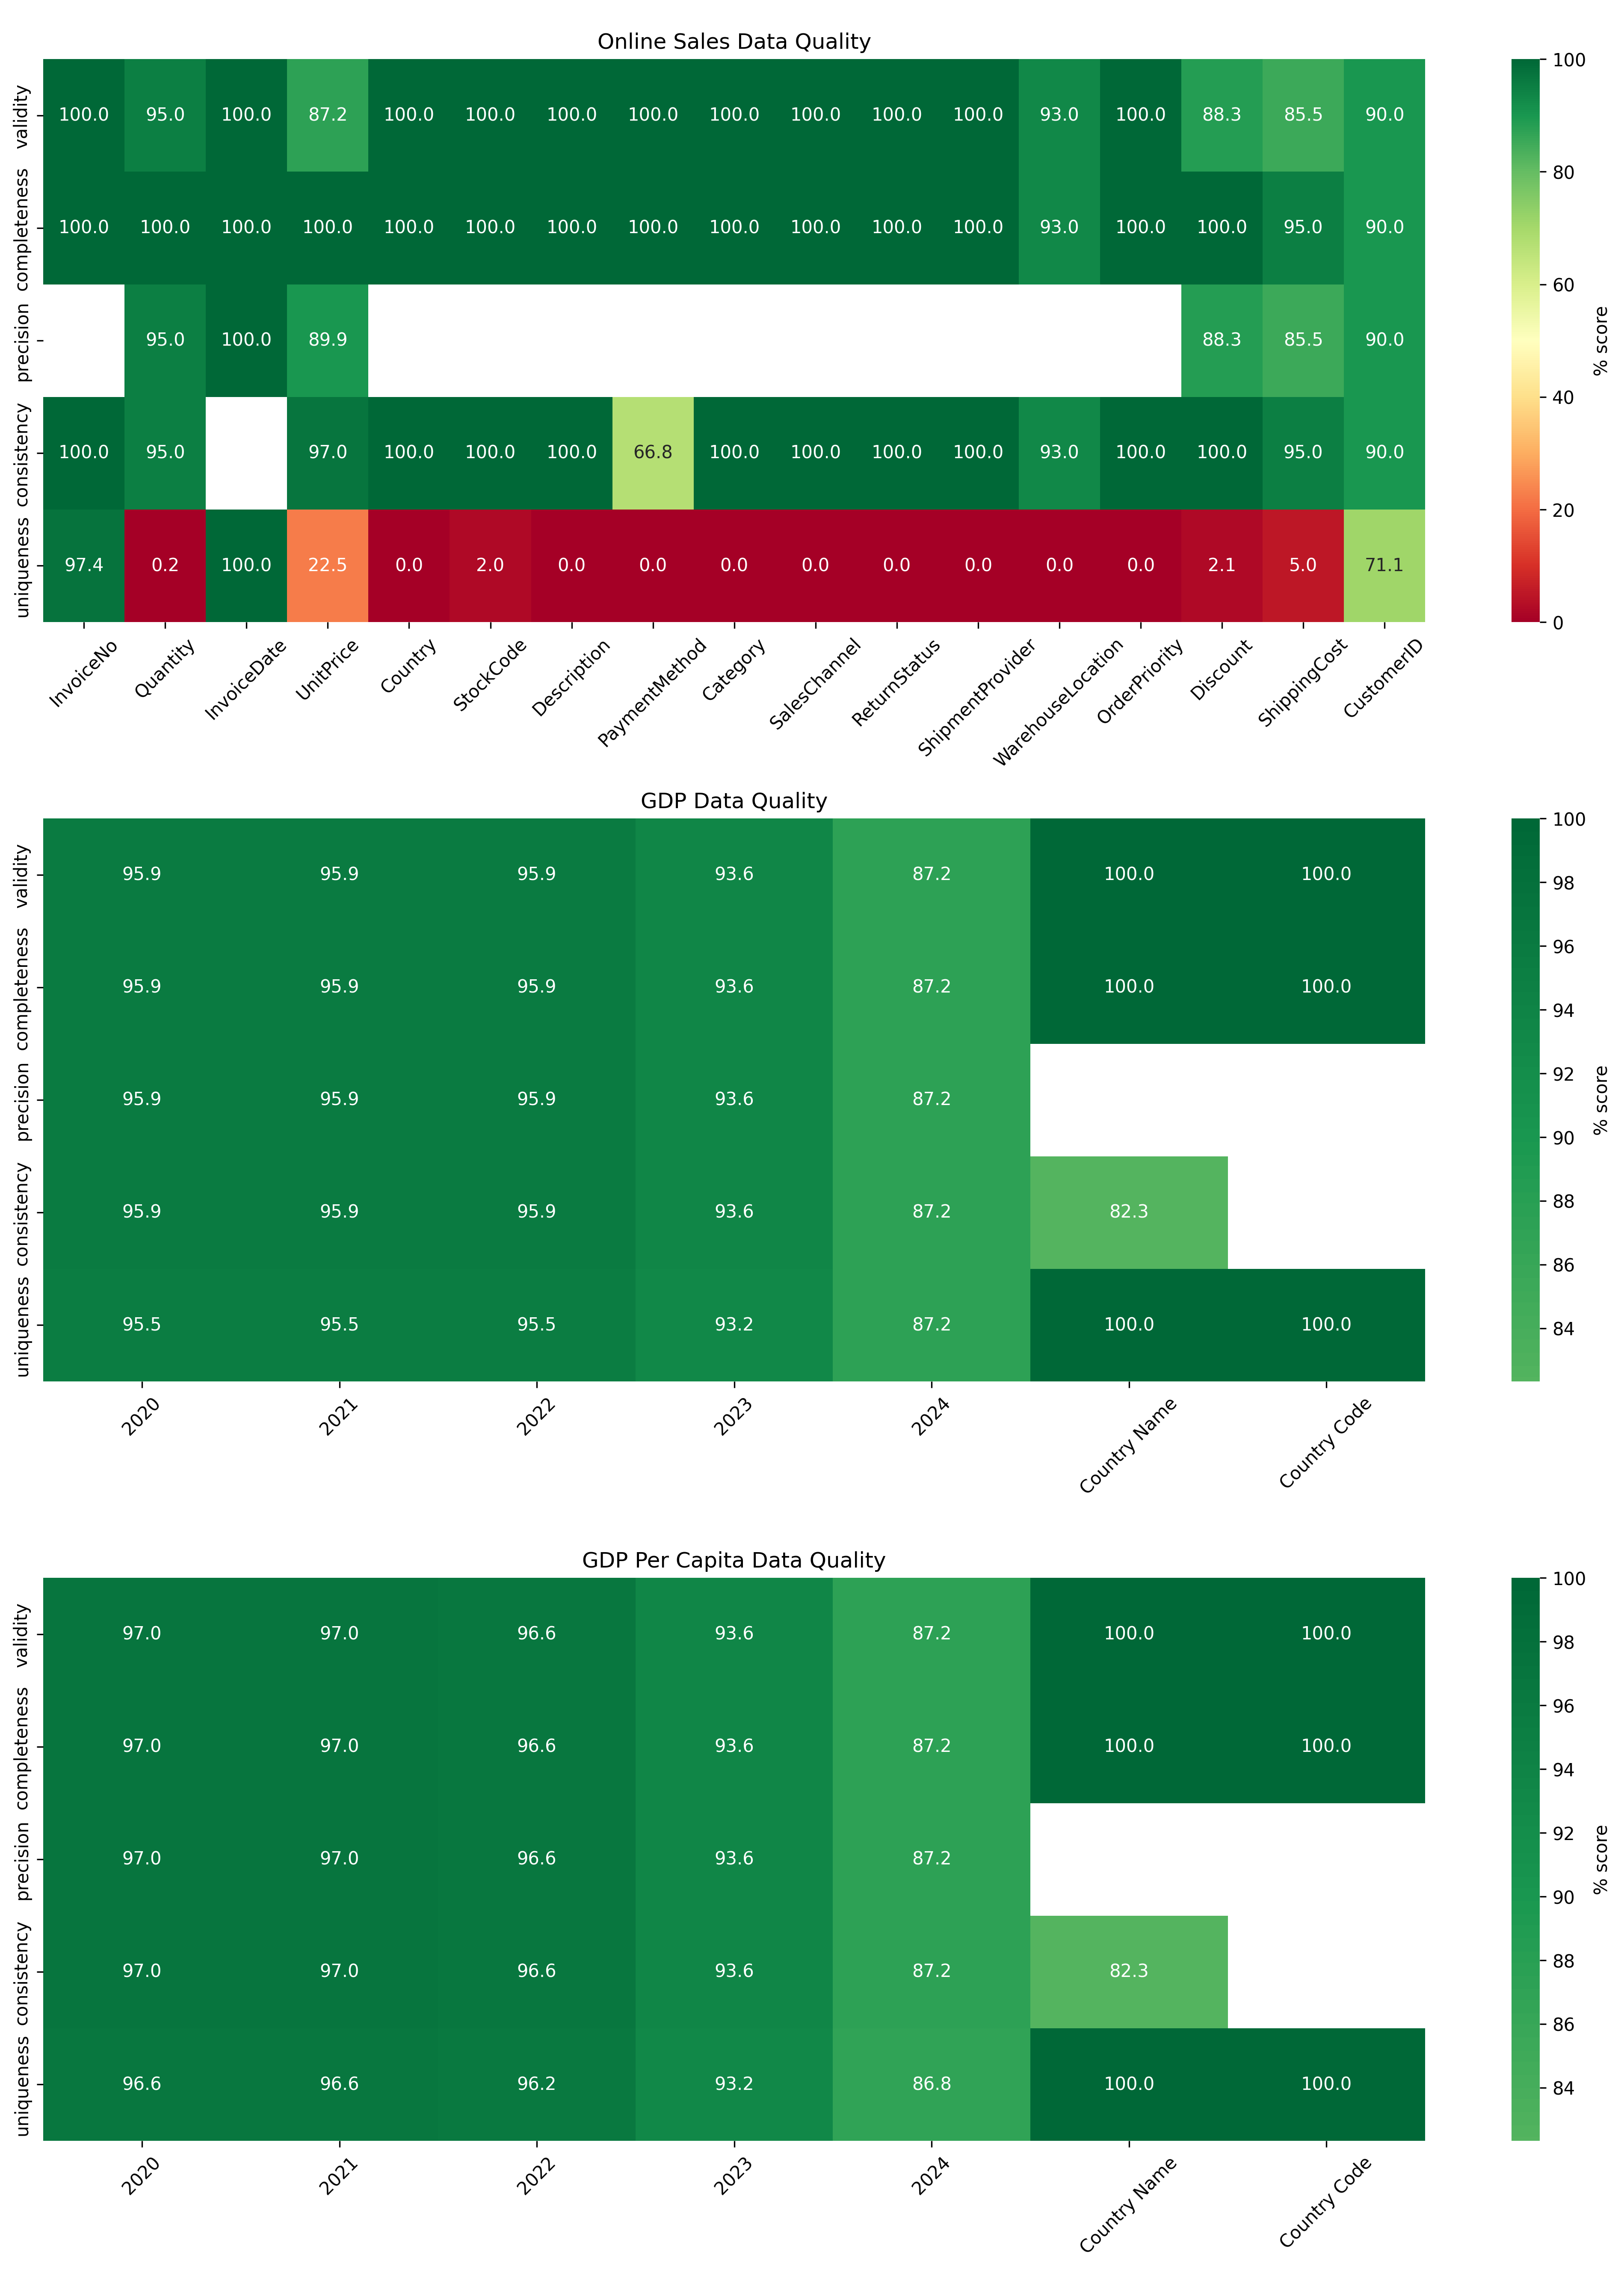
\includegraphics[width=0.85\textwidth]{../Visualizations/Pre/PRE_combined_heatmap.png}
    \caption{Initial data quality assessment heatmap for the Online Sales Dataset.}
    \label{fig:initial_data_quality_heatmap}
\end{figure}

\textbf{Online Sales Dataset Quality Issues:}
\begin{itemize}
    \item \textbf{Validity violations}: Fields such as \texttt{Quantity} and \texttt{UnitPrice} contained invalid negative values; \texttt{PaymentMethod} showed typographical errors; \texttt{ShipmentProvider}, \texttt{Discount}, and \texttt{ShippingCost} suffered from inconsistent formats.

    \item \textbf{Completeness issues}: Missing values were present in various fields.

    \item \textbf{Precision anomalies}: Numerical fields exhibited incorrect decimal formatting and inconsistent precision.

    \item \textbf{Consistency Problems}: The allegedly synthetic nature of the dataset resulted in random and inconsistent values.
\end{itemize}
\textbf{World Bank Economic Data Quality Issues:}
The GDP datasets exhibited data gaps primarily in small nation-states and recent years where official statistics had not yet been published.

\section{Data Integration with World Bank Economic Indicators}

\subsection{World Bank Economic Data Processing}

The \texttt{2\_Pulizia\_CSV\_GDP.py} script was used to rescale World Bank GDP datasets in a consistent manner.
The time period was filtered for values between 2020-2024, matching the range of the Online Sales Dataset. \\
Data quality improvement handling missing values in one of these two ways:
\begin{itemize}
    \item Linear interpolation was applied where there was minimal missing data to impute missing values
    \item Those with over two years of consecutive missing data were removed in an attempt to maintain continuity
\end{itemize}

\subsection{Data Cleaning and Preparation Process}

The raw datasets required extensive cleaning before integration.

\begin{enumerate}
    \item  \textbf{Online Sales Dataset Cleaning}\\
    Regular expressions were used to filter the correct values.
    Negative values in numerical fields were deleted or changed in absolute value depending on the type of field.
    The \texttt{Discount} column was normalized between 0 and 1.\\
    Text standardization corrected common typos and ensured consistent formatting for InvoiceNo and \texttt{StockCode} values.
    A new column \texttt{EstimatedUnitCost} was added, calculated as a random variation of the \texttt{UnitPrice} to simulate a plausible price of the items and calculate more meaningful KPI's with ease.
    A significant enhancement was creating realistic multi-item orders.
    The original dataset contained mostly single-item transactions, but with repeating InvoiceNumbers due to its allegedly random-generation nature, so related items were grouped into single multi-article orders

    \item \textbf{Economic Data Integration}\\
    Integrating the World Bank economic indicators required a careful alignment between the two datasets. 
    The destination countries of the customers in the Online Sales Dataset (OSD) were matched with the countries in the GDP CSV file, using their respective ISO alpha-3 codes to simplify representation with a standardized one.
    Wherever economic data were missing they were handled as previously mentioned.
\end{enumerate}
\textbf{Final Dataset Quality}
The cleaning process transformed the original 49,782 records into a refined dataset of 43,434 records significantly improving data quality.

\begin{figure}
    \centering
    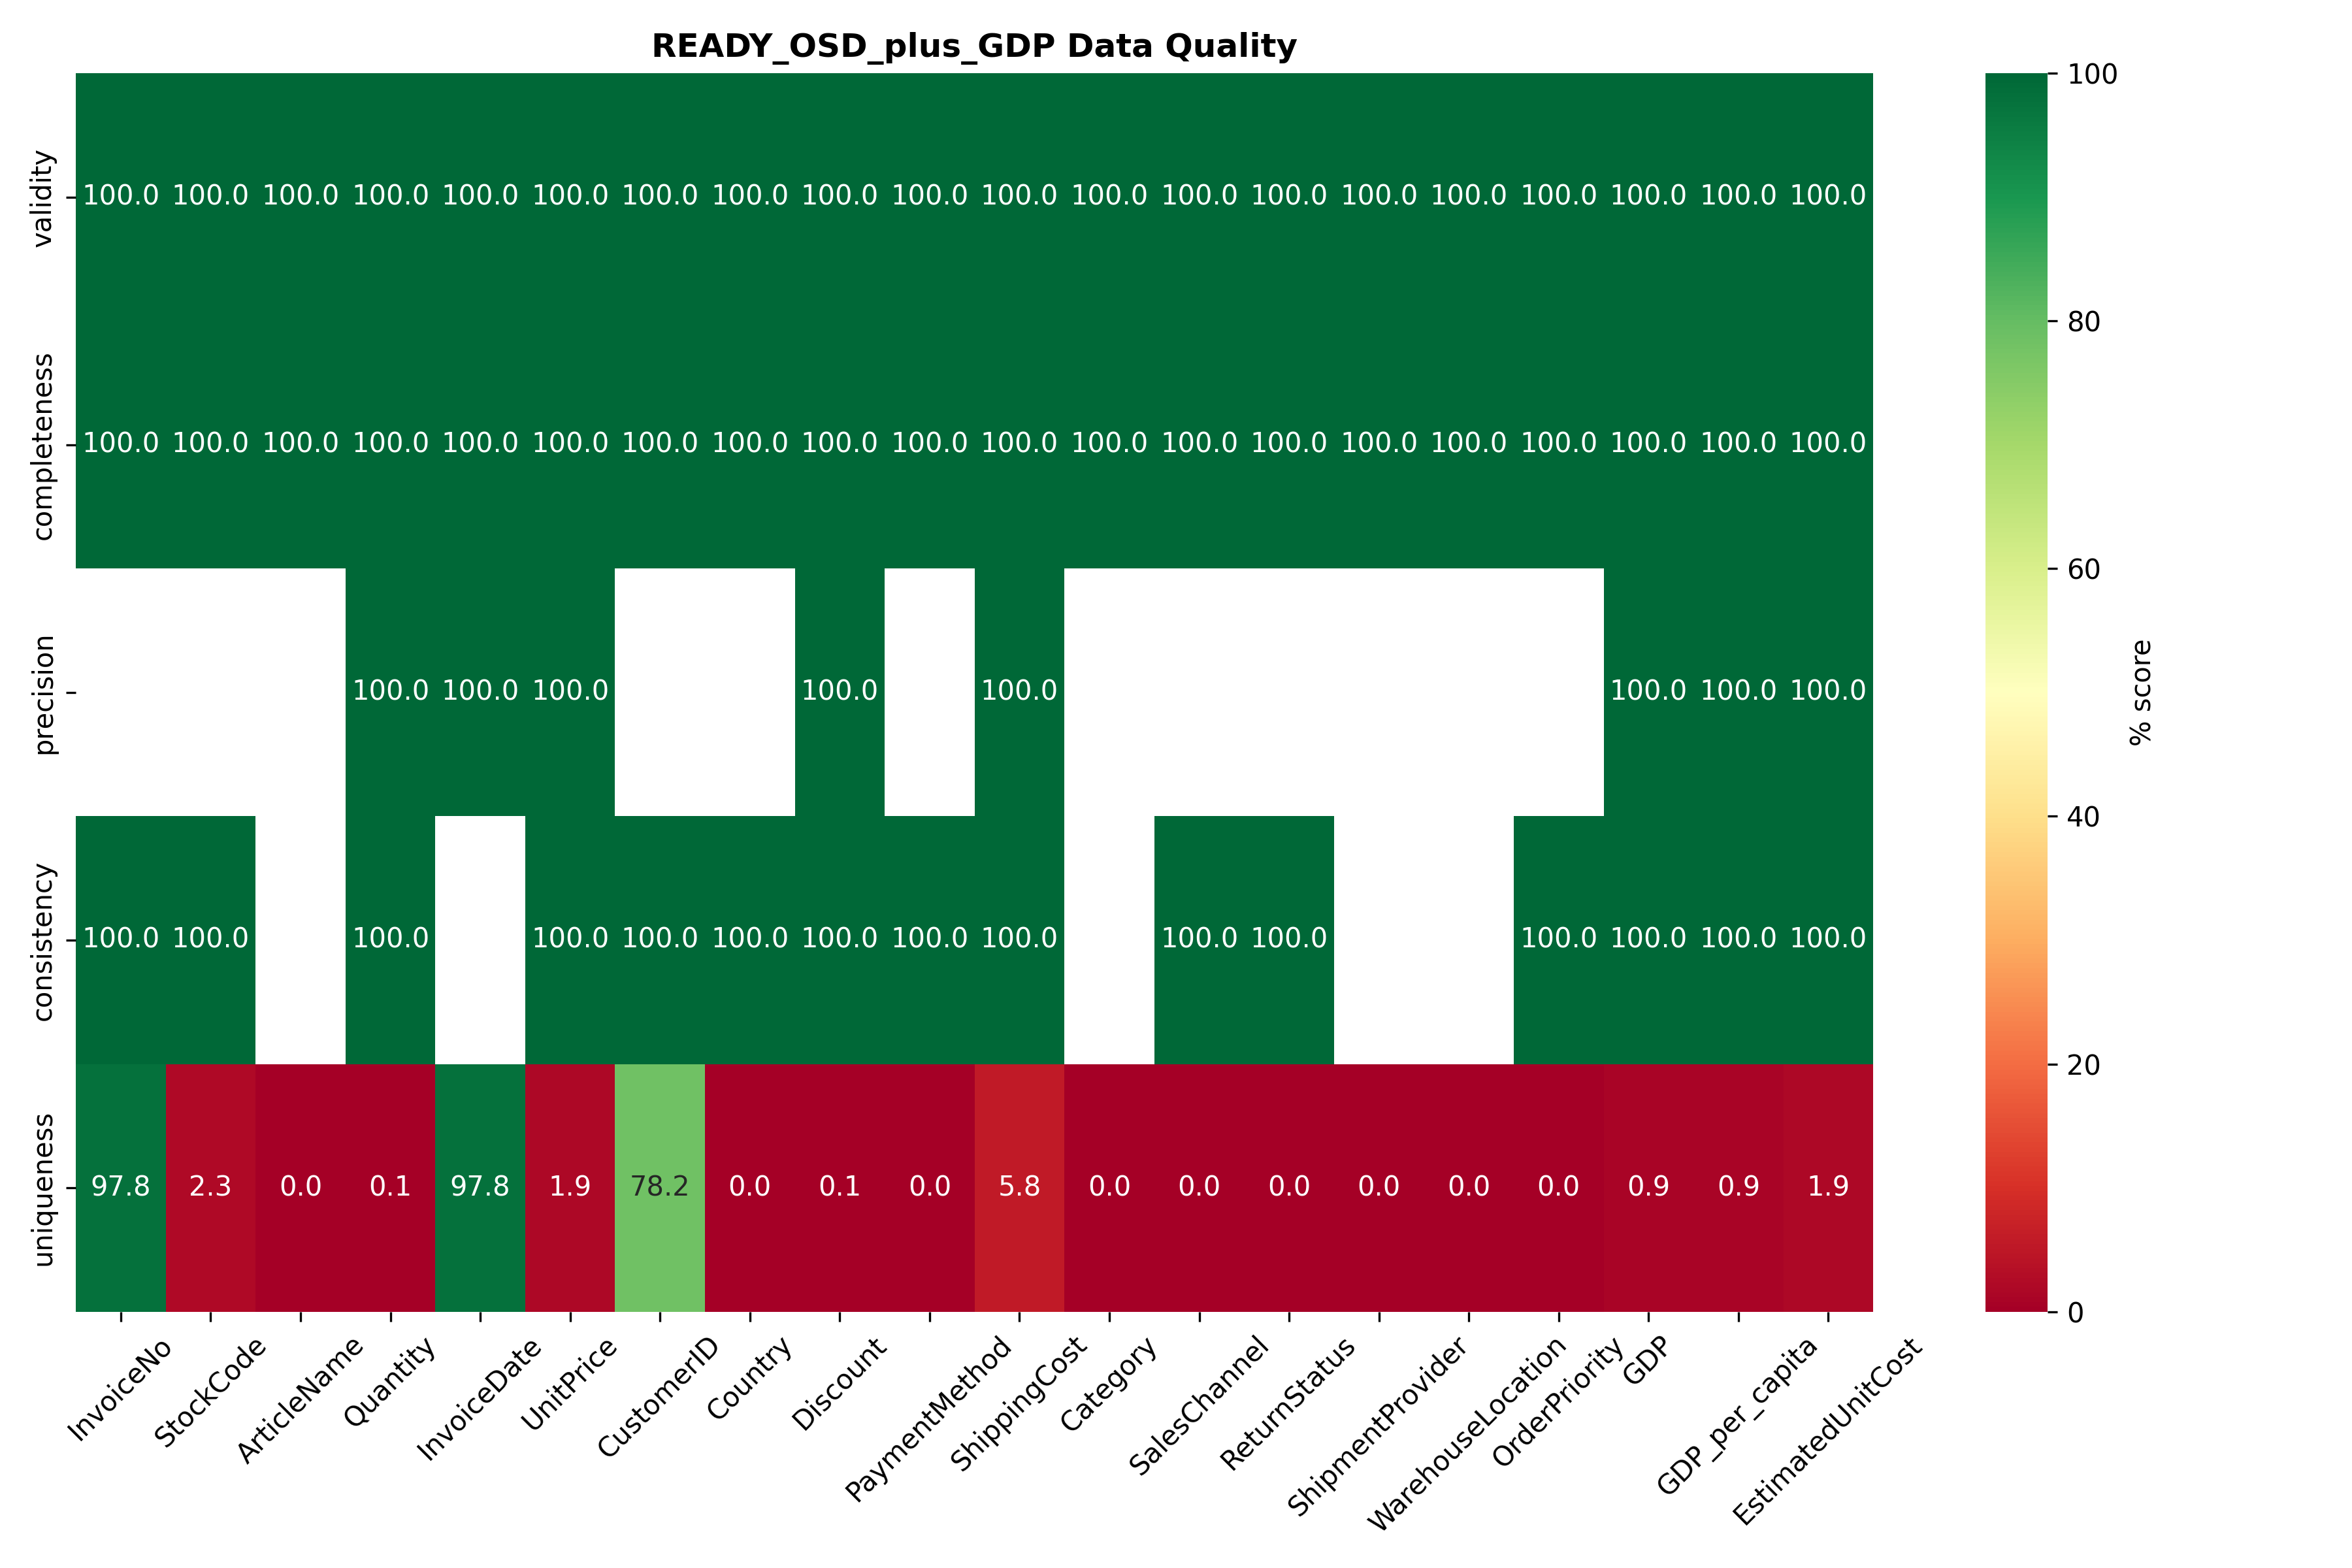
\includegraphics[width=0.85\textwidth]{../Visualizations/Post/POST_OSD_plus_GDP_heatmap.png}
    \caption{Final data quality assessment heatmap for the cleaned Online Sales Dataset + GDP.}
    \label{fig:final_data_quality_heatmap}
\end{figure}

\section{Conceptual and Logical Schema}

\subsection{Initial E/R Schema}
\begin{figure}[H]
\centering
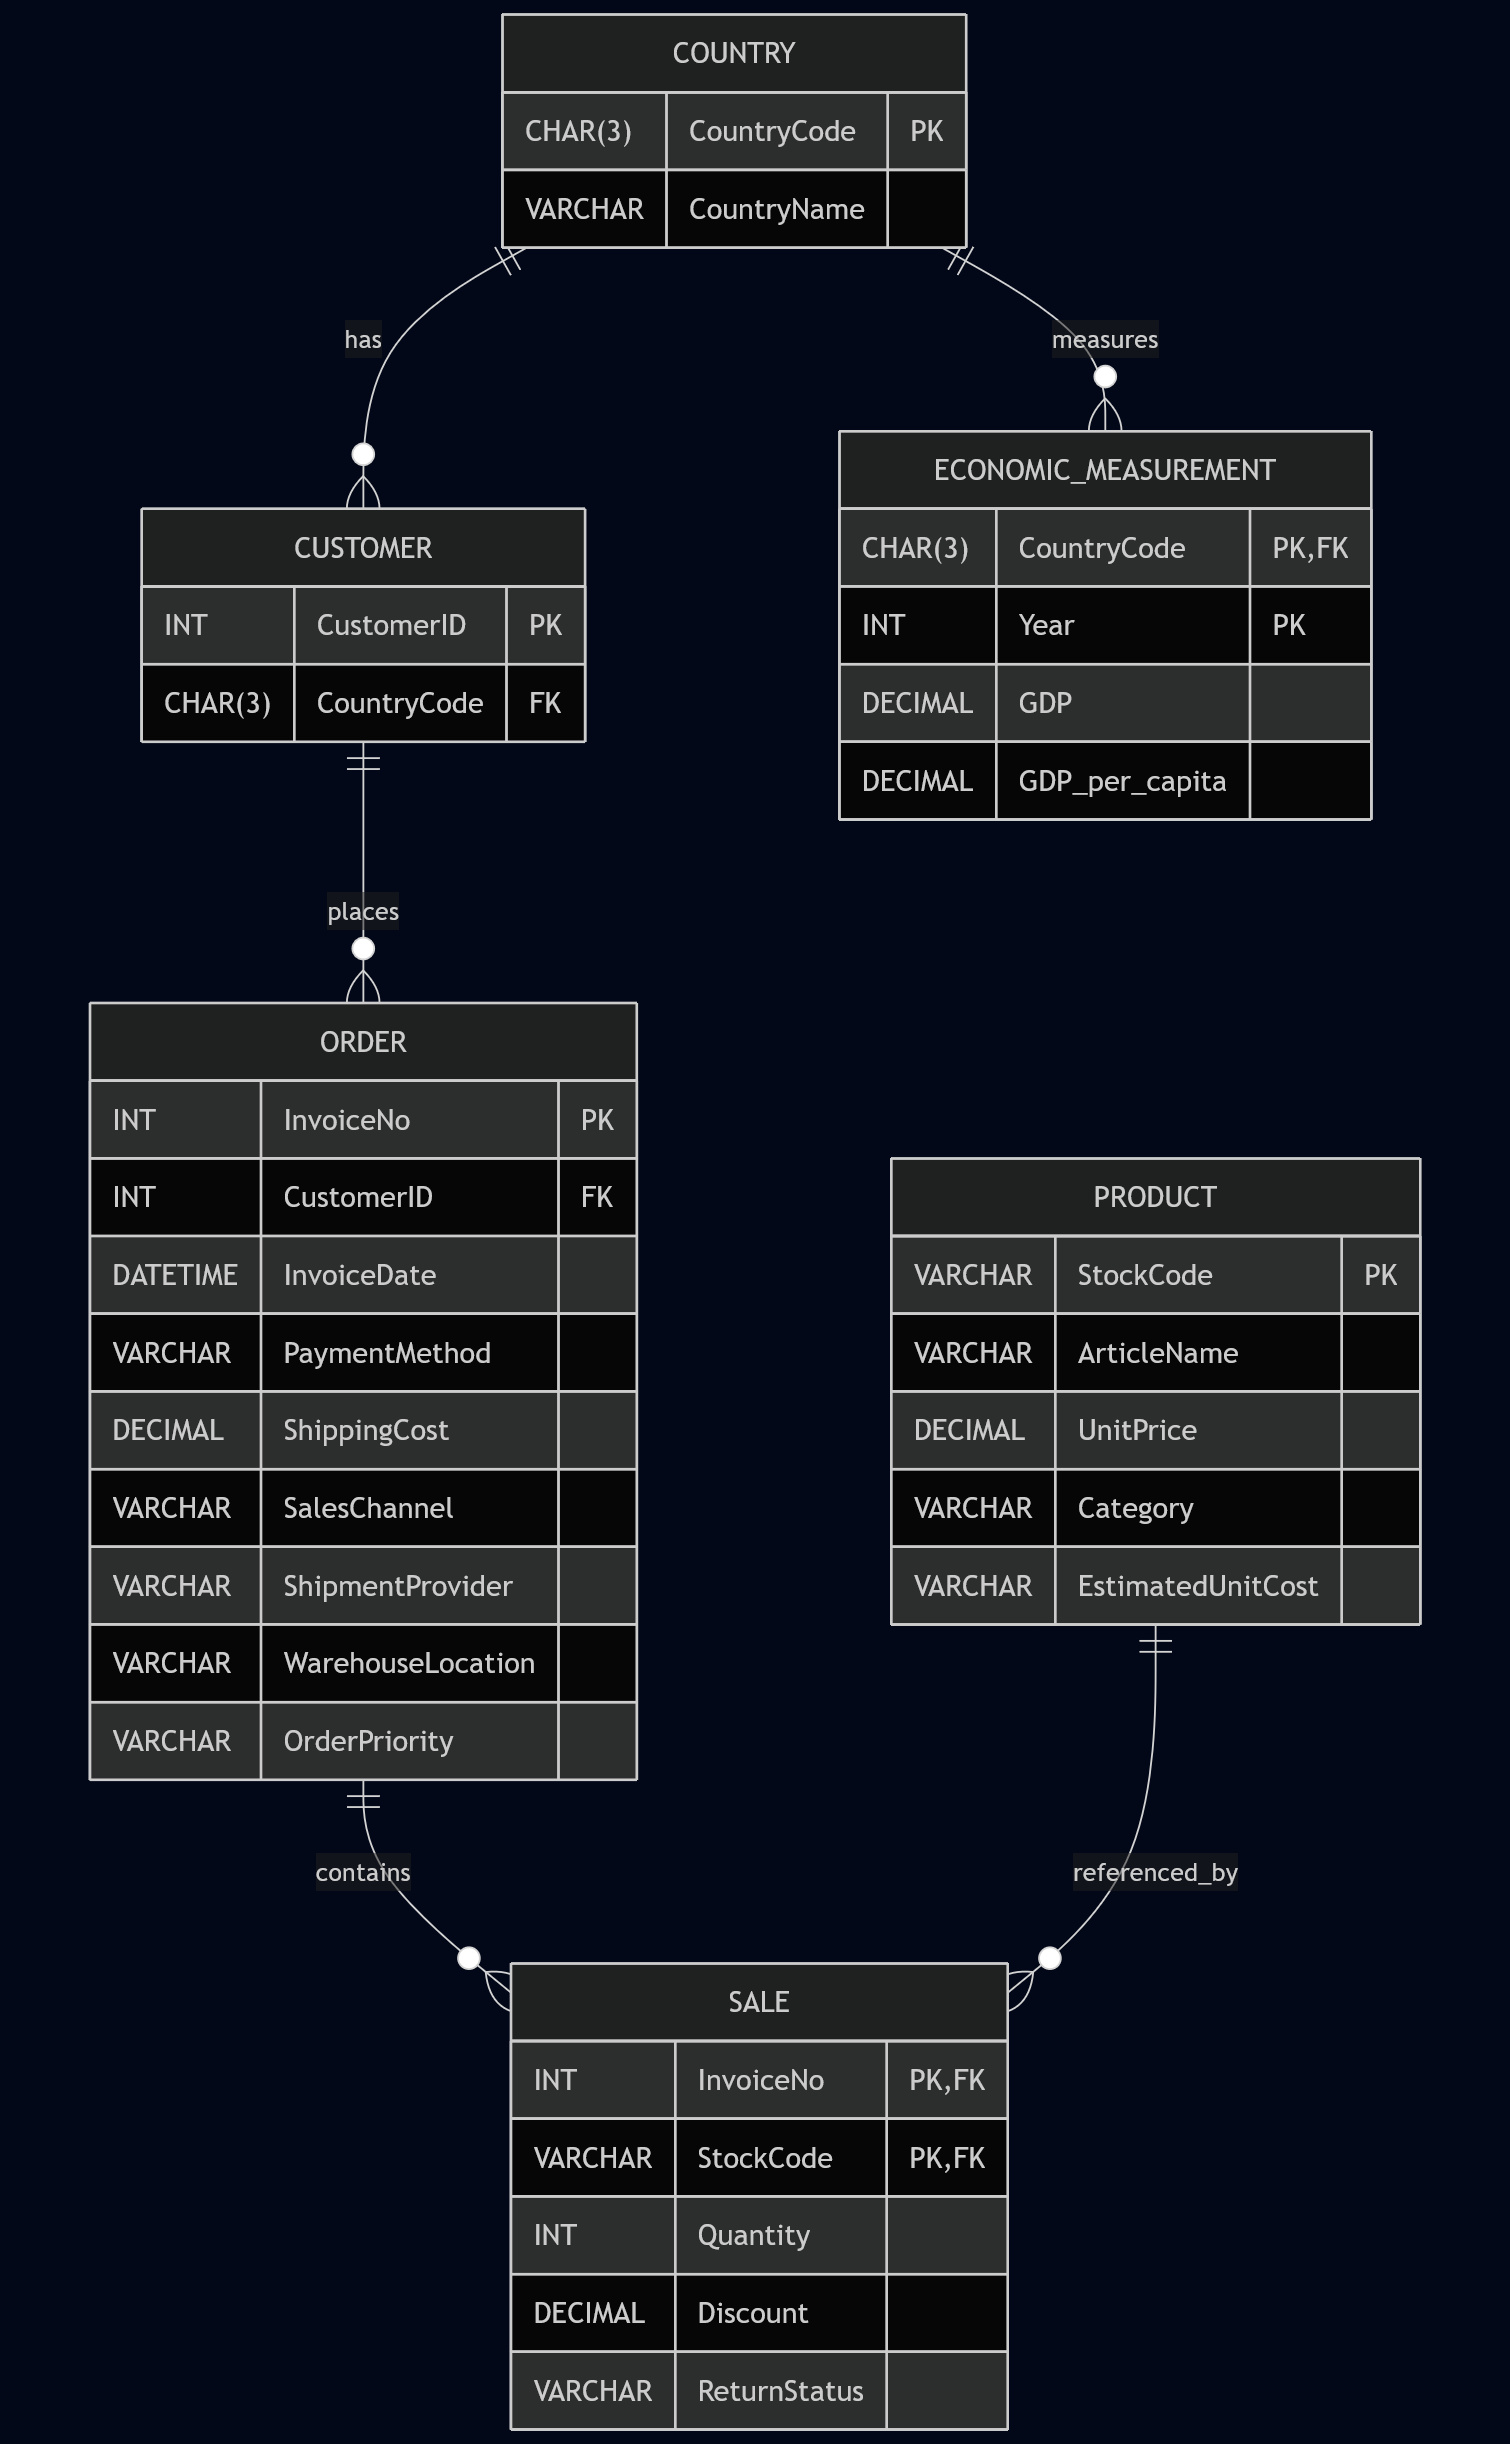
\includegraphics[width=0.9\textwidth]{../Graphs/0_Schema_ER.png}
\caption{Initial Entity-Relationship diagram of the \textit{Online Sales Dataset}.}
\label{fig:initial_er_schema}
\end{figure}

The central entities in the first E/R model are: \textbf{Sale}, \textbf{Order}, \textbf{Product}, \textbf{Customer}, \textbf{Country}, and \textbf{Economic\_Measurement}.
\texttt{Order} is central in the schema: each Order is associated with one or more \texttt{Sale} entries, each linked to a \texttt{Product}.
The Geo-Economical situation is addressed by the \texttt{Customer}-\texttt{Country} and the \texttt{Economic\_Measurement} entity which provides GDP context for each country.

\subsection{Attribute Tree}
\begin{figure}[H]
\centering
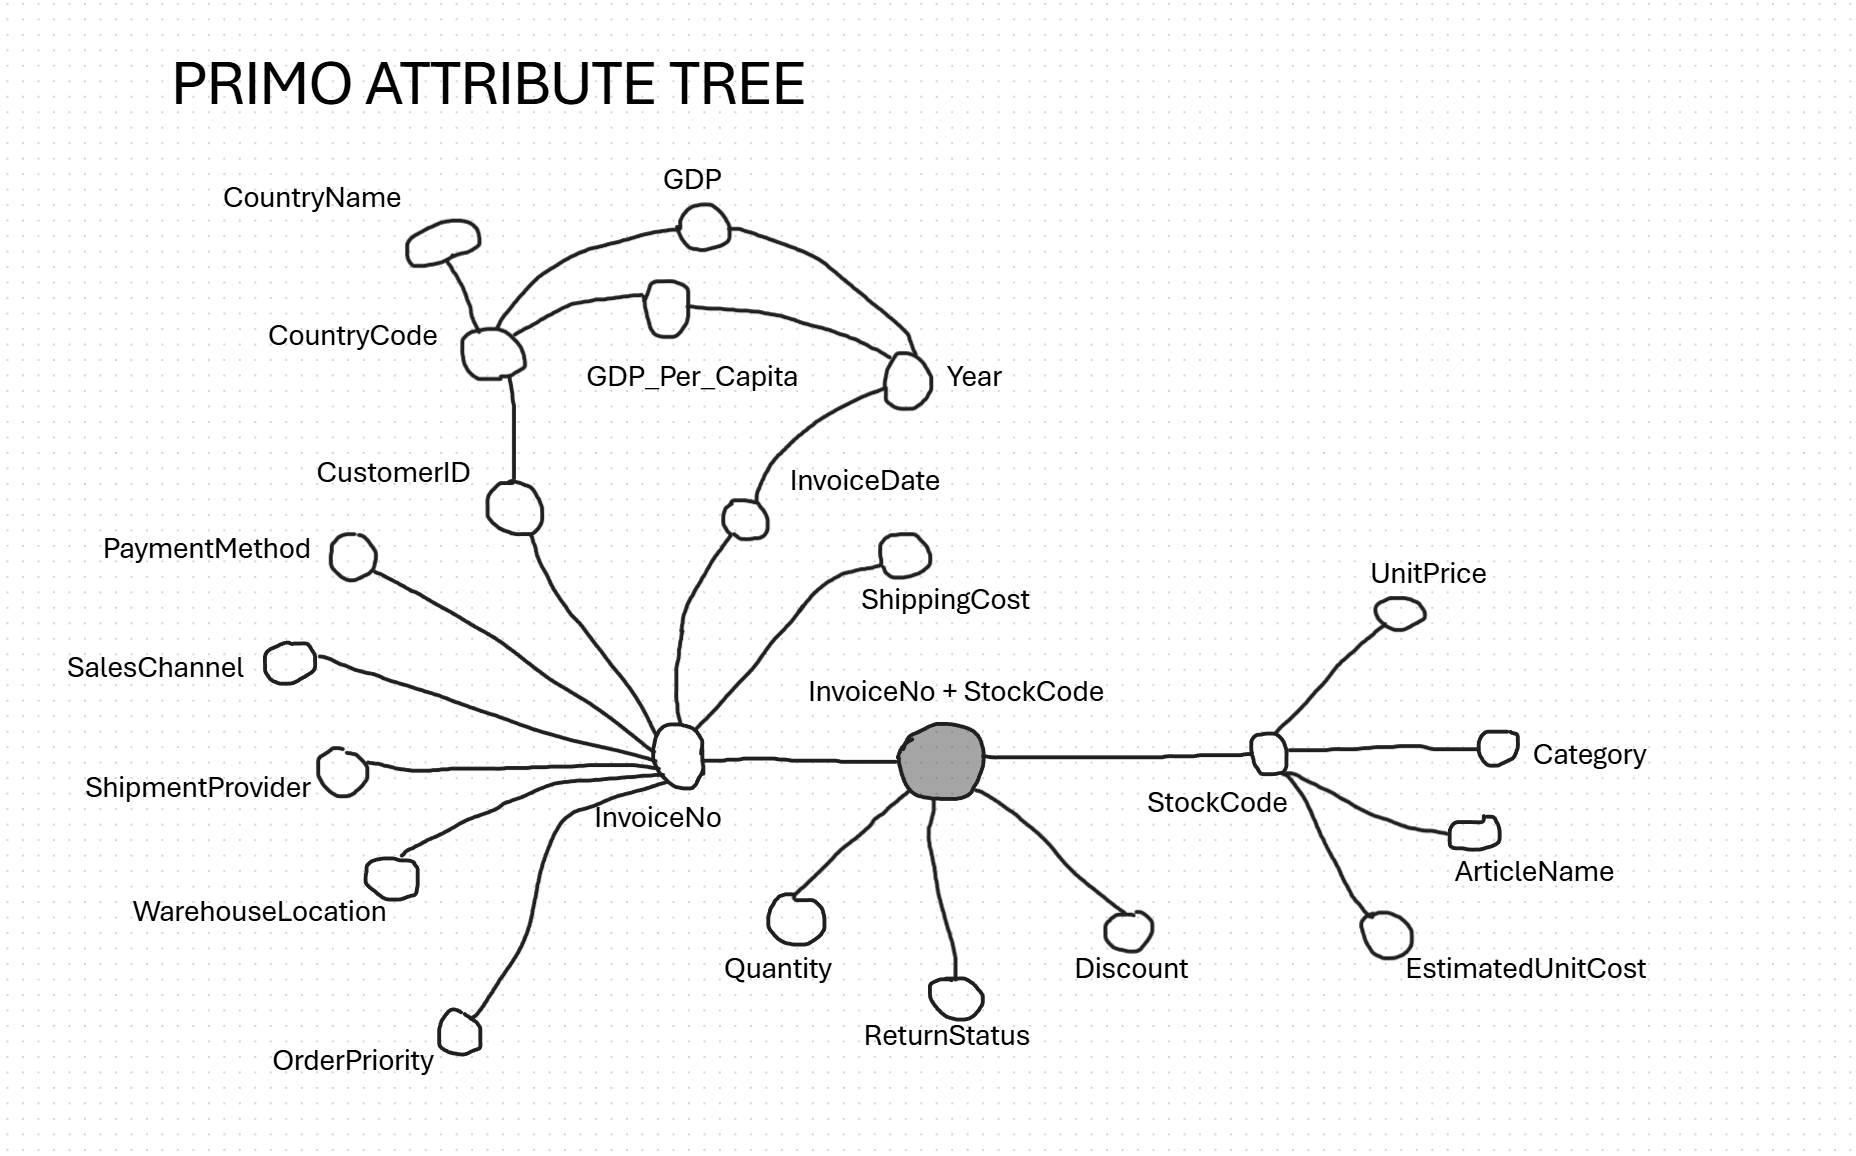
\includegraphics[width=0.85\textwidth]{../Graphs/1_Attribute_Tree.png}
\caption{Attribute tree — full version.}
\label{fig:attribute_tree_full}
\end{figure}

\textbf{Step 1 - initial attribute tree}: all the raw dataset attributes were mapped giving a complete but rough idea of the data available. 

\begin{figure}[H]
\centering
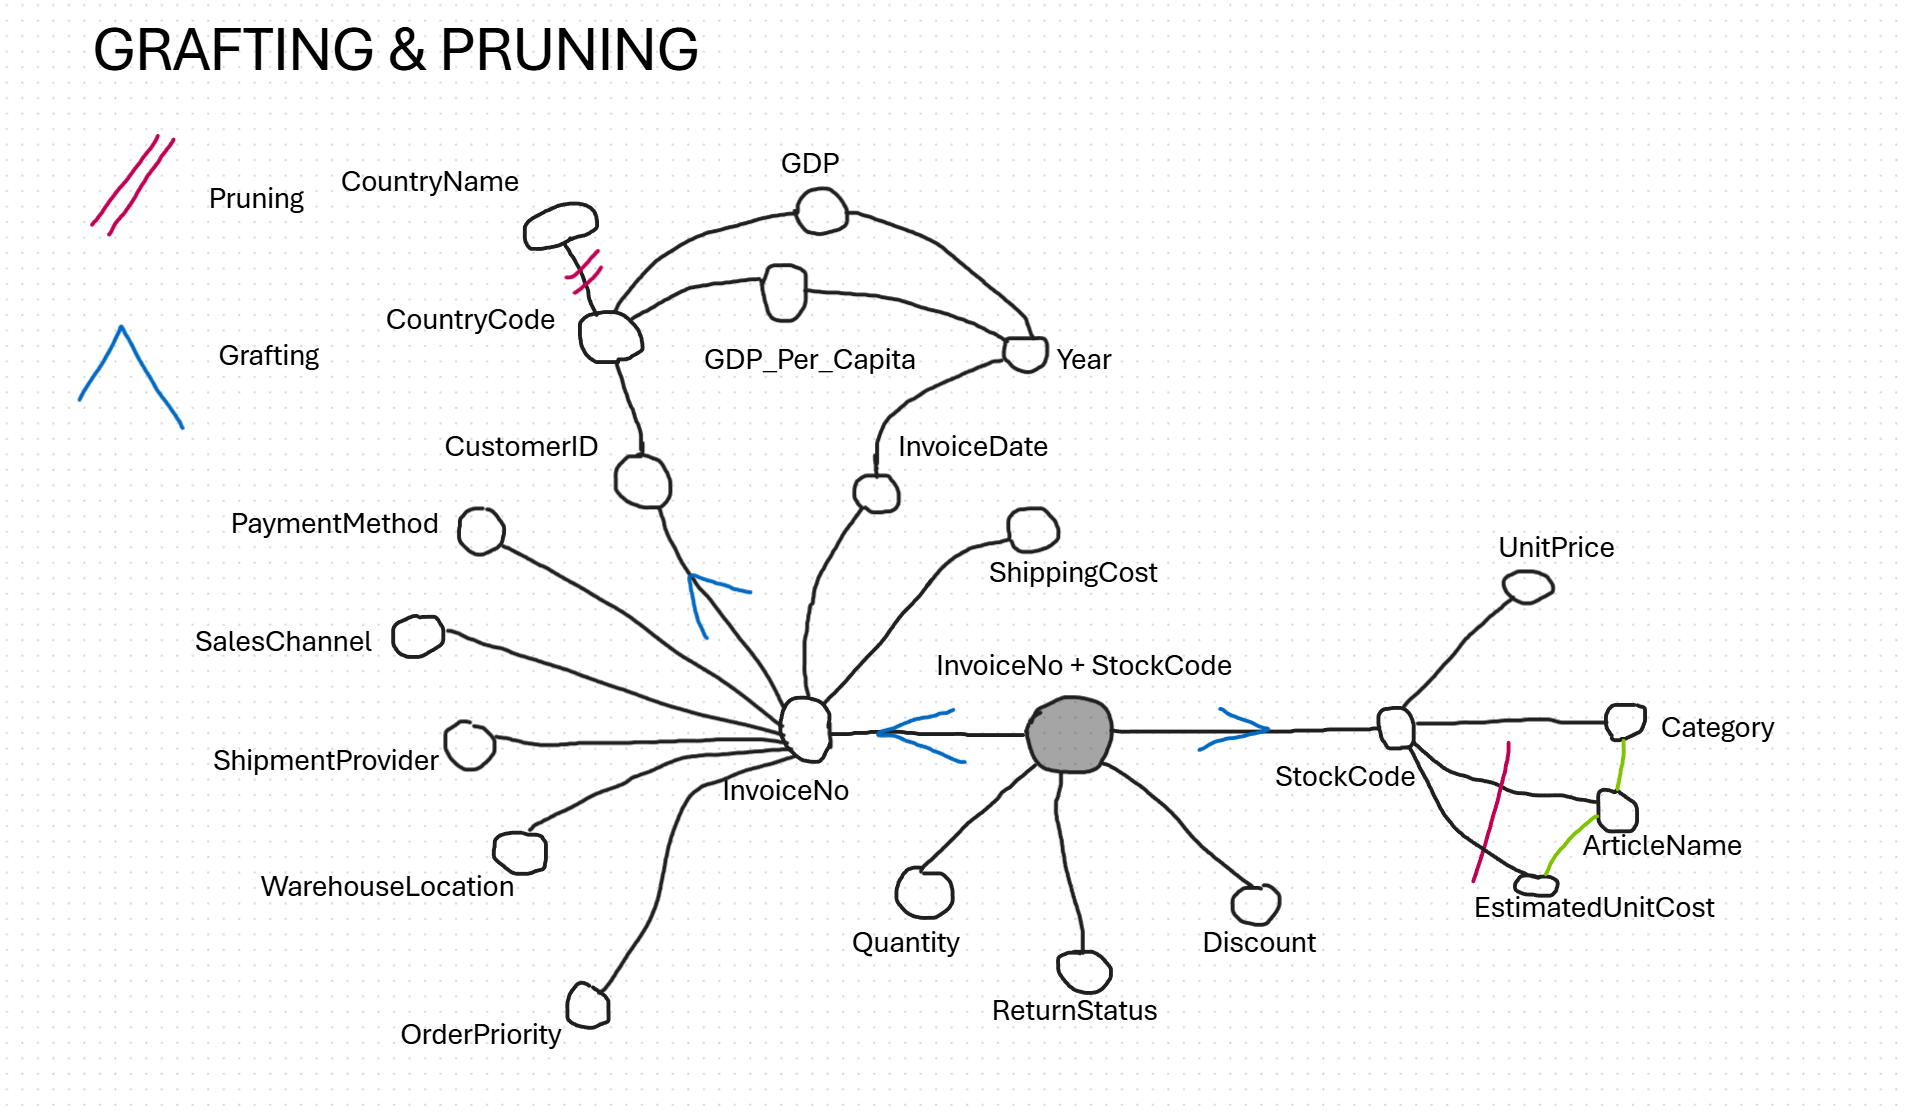
\includegraphics[width=0.85\textwidth]{../Graphs/2_Attribute_Tree_Pruning_Grafting.png}
\caption{Pruning and grafting of the attribute tree.}
\label{fig:attribute_tree_pruning_grafting}
\end{figure}

\textbf{Step 2 - pruning and grafting}: Attributes such as \texttt{InvoiceNo}, \texttt{StockCode}, and \texttt{CustomerID} were grafted into the tree root as they didn't add particular analytical value.
The \texttt{CountryName} attribute was pruned as \texttt{CountryCode} is sufficient to uniquely identify countries.
Additionally, \texttt{ArticleName} was repositioned as part of the hierarchy under \texttt{Category}, rather than being directly linked to \texttt{StockCode}.

\begin{figure}[H]
\centering
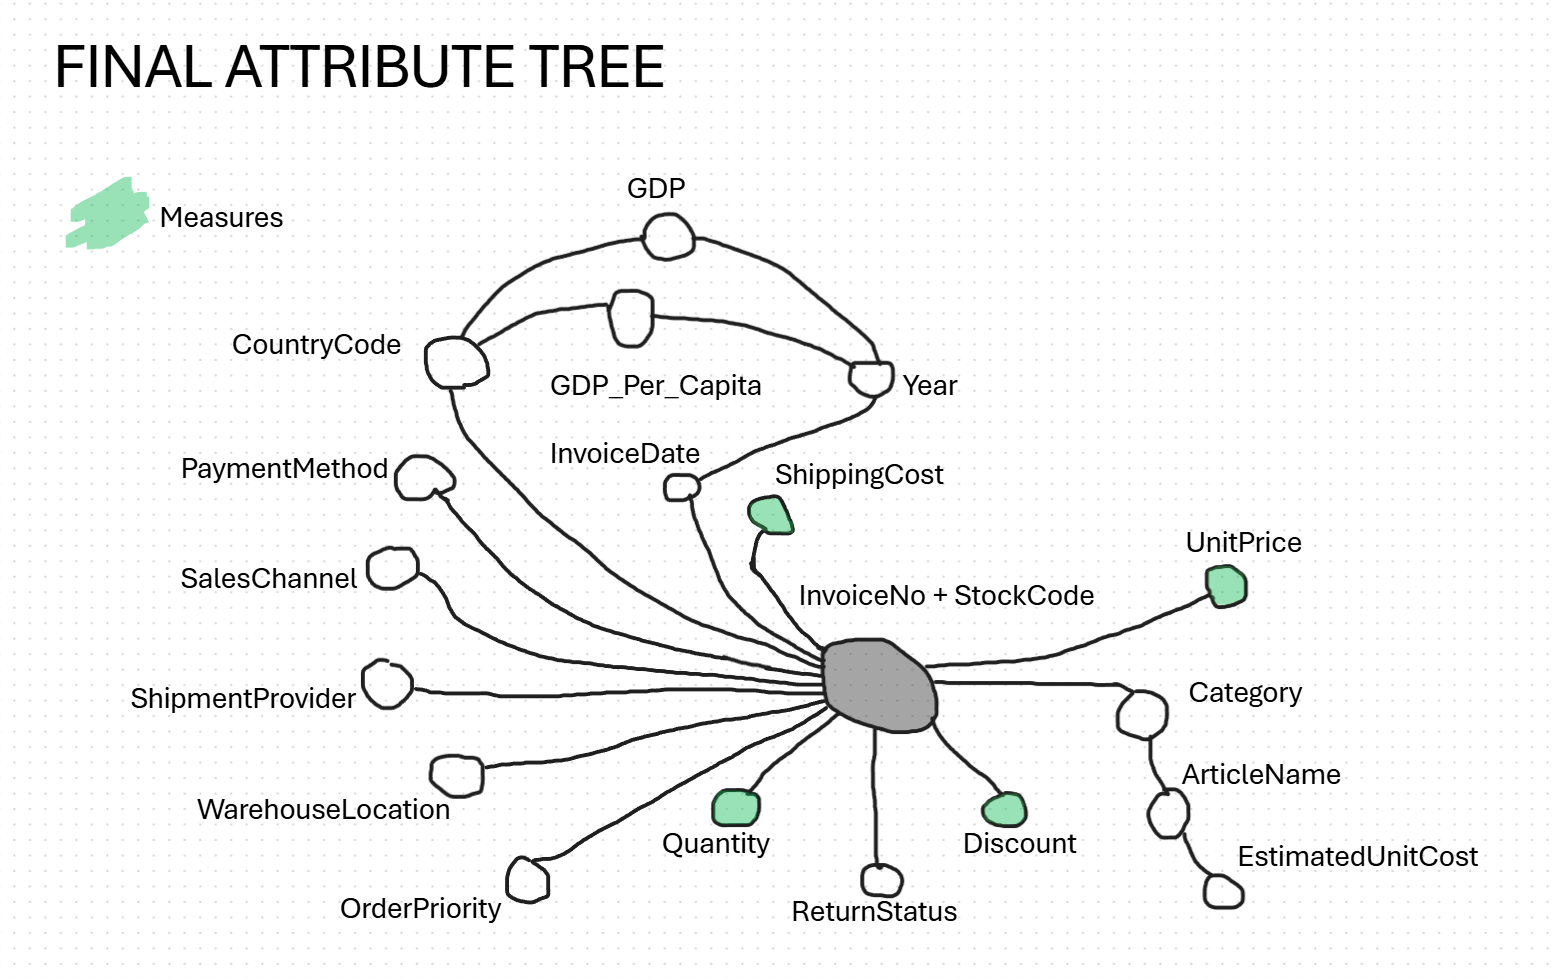
\includegraphics[width=0.85\textwidth]{../Graphs/3_Final_Attribute_Tree.png}
\caption{Final attribute tree.}
\label{fig:final_attribute_tree}
\end{figure}

\textbf{Step 3 - final version}: the final attribute tree contains only the attributes relevant for analytical purposes.

\clearpage

\subsection{Dimensional Fact Model}
\begin{figure}[H]
\centering
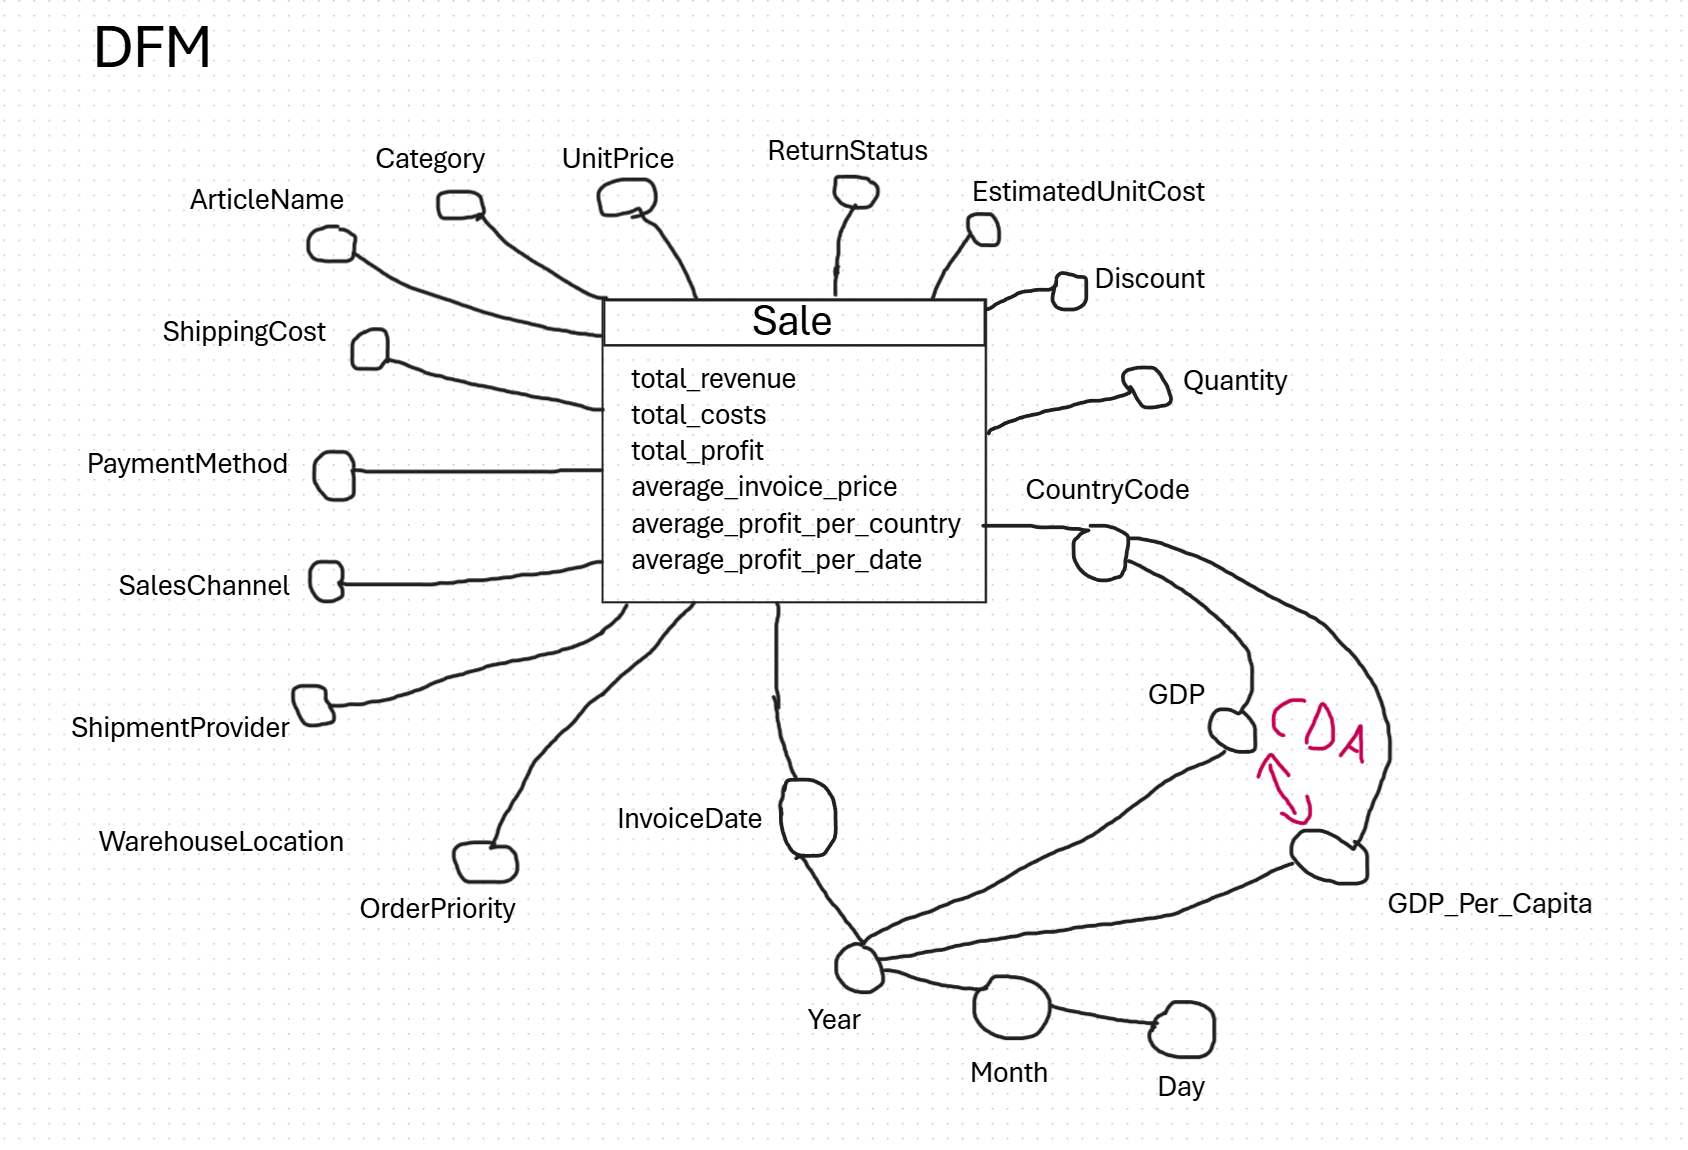
\includegraphics[width=0.85\textwidth]{../Graphs/4_Dimensional_Fact_Model.png}
\caption{Dimensional Fact Model.}
\label{fig:dimensional_fact_model}
\end{figure}

Given the final attribute tree, the dimensional fact model was created.
The \texttt{Sales} table is the central fact table, containing measures such as \texttt{TotalRevenue}, \texttt{TotalCost}, and \texttt{TotalProfit} etc.

\subsection{Star Schema}
\begin{figure}[H]
\centering
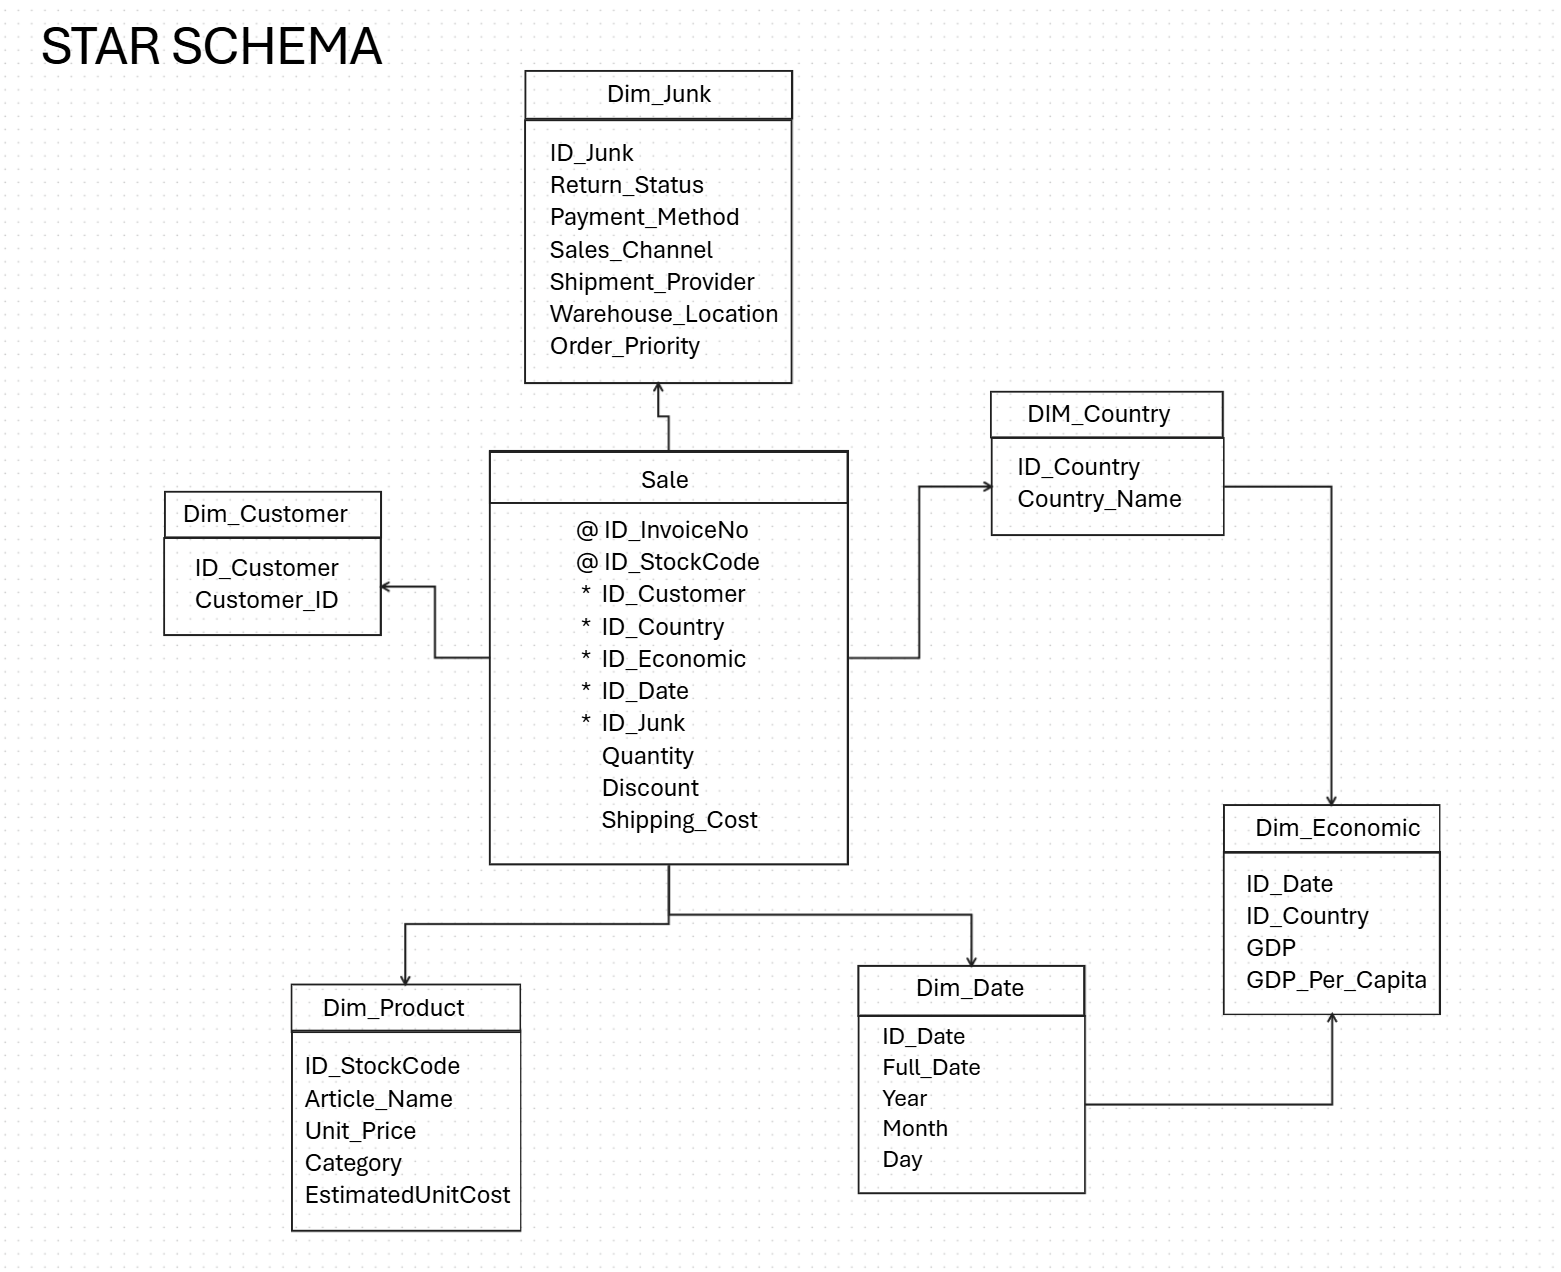
\includegraphics[width=0.85\textwidth]{../Graphs/5_Star_Schema.png}
\caption{Final Star Schema of the Data Warehouse.}
\label{fig:star_schema}
\end{figure}

To avoid having many degenerate dimension we created a Junk one, \texttt{Dim\_Junk}, to group attributes such as (e.g., \texttt{Return\_Status}, \texttt{Sales\_Channel}, \texttt{Payment\_Method}) into a compact structure.
The \texttt{Dim\_Economic} dimension, linked via \texttt{ID\_Country} and \texttt{ID\_Date}, enables geo-economic analyses by correlating KPIs with GDP and GDP per capita over time.


\begin{thebibliography}{99}
\bibitem{osd} \url{https://www.kaggle.com/datasets/yusufdelikkaya/online-sales-dataset}
\bibitem{wb1} \url{https://data.worldbank.org/indicator/NY.GDP.MKTP.KD}
\bibitem{wb2} \url{https://data.worldbank.org/indicator/NY.GDP.PCAP.CD}
\bibitem{er_diagram} \url{https://github.com/PierpaoloSpadafora/Data_Warehouse}
\end{thebibliography}


\end{document}